\documentclass[titlepage,11pt]{article}
\usepackage{comment}
\usepackage{enumitem}
\usepackage{transparent} % Untuk transparansi gambar
\usepackage{listings}
\usepackage{amsmath}
\usepackage{graphicx}
\usepackage[font=small,labelfont=bf]{caption}
\usepackage[bahasa]{babel}
\usepackage{float}
\usepackage{verbatim}
\usepackage{graphicx,tabularx,multirow}
\usepackage{xcolor}
\usepackage[onehalfspacing]{setspace}
\usepackage[
	allcolors=visigrey,
	colorlinks=true,
]{hyperref}
\usepackage[a4paper,left=2cm,right=2cm]{geometry}
% Pengaturan kutipan artikel
\usepackage[style=ieee, backend=biber]{biblatex}
%Code listing style pak akok
\definecolor{codegreen}{rgb}{0,0.6,0}
\definecolor{codegray}{rgb}{0.5,0.5,0.5}
\definecolor{codepurple}{rgb}{0.58,0,0.82}
\definecolor{backcolour}{rgb}{0.95,0.95,0.92}

\usepackage{eso-pic} % Untuk menambahkan elemen ke seluruh halaman

\newcommand\BackgroundPic{
  \put(0,0){
    \parbox[b][\paperheight]{\paperwidth}{
      \vfill
      \centering
      \transparent{0.1}
      \includegraphics[width=0.4\paperwidth,keepaspectratio]{miot.png}
      \vfill
    }
  }
}

\newcommand\BackgroundAllPages{ \AddToShipoutPicture*{\BackgroundPic} }
\newcommand\BackgroundNone{ \ClearShipoutPicture } % hilangkan background

\lstdefinestyle{mystyle}{
	backgroundcolor=\color{backcolour}, commentstyle=\color{codegreen},
	keywordstyle=\color{magenta},
	numberstyle=\small\color{codegray},
	stringstyle=\color{codepurple},
	basicstyle=\ttfamily\footnotesize,
	breakatwhitespace=false,         
	breaklines=true,                 
	captionpos=t,                    
	keepspaces=true,                 
	numbers=left,                    
	numbersep=5pt,                  
	showspaces=false,                
	showstringspaces=false,
	showtabs=false,           
	frame = single,
	tabsize=2
}
\lstset{style=mystyle}

\definecolor{visigrey}{rgb}{.1,.15,.15}
\geometry{top=1cm,bottom=.5cm}
\savegeometry{titlepage}
\geometry{top=2cm,bottom=2cm}
\savegeometry{main}

\def\bspace{\(\qquad\qquad\qquad\)}
\usepackage[T1]{fontenc}
\usepackage[utf8]{inputenc}
\usepackage{tgheros}
\renewcommand*\familydefault{\sfdefault}

\setcounter{tocdepth}{6}

\def\autor{Laboratorium }
\def\lab{Multimedia dan Internet of Things}
\def\departemen{Departemen Teknik Komputer}
\def\institut{Institut Teknologi Sepuluh Nopember}
\def\praktikum{Laporan Sementara \\ Praktikum Jaringan Komputer}
\def\nama{Bintang Narindra Putra Pratama - 5024231038}
% Ubah Judul sesuai dengan modul
\def\judul{Firewall dan NAT}
\def\tanggal{2025}
\begin{document}
% Ubah Bahasa sesuai dengan keinginan
\selectlanguage{bahasa}

\BackgroundNone
\def\headingtype{\bf \small}
\loadgeometry{titlepage}

\begin{titlepage}
	\centering
	\begin{tabularx}{\textwidth}{l@{\hskip 0pt}lX}
		\raisebox{-0.5\height}{
\includegraphics[width=3cm]{Cover/img/logodepart.png}} 
		& \raisebox{-0.5\height}{\includegraphics[width=3cm]{Cover/img/miot.png}} 
		& \raggedleft
	\hfill
	\begin{minipage}{0.5\textwidth}
		\raggedleft
		{\emph{\headingtype \autor}} \\[-2pt]
		{\headingtype \lab} \\[-2pt]
		{\headingtype \departemen} \\[-2pt]
		{\headingtype \emph{\institut}}
	\end{minipage}

	\vspace{5cm}
	\end{tabularx}
	
	\vspace{5cm}
	{\Huge \bf \praktikum \par}
	
	\vspace{2cm}
	{\LARGE \bf \judul \par}
	
	\vspace{2cm}
	{\Large \nama \par}
	
	\vfill
	{\Large \tanggal \par}
	
	\vfill
	
\includegraphics[width=\textwidth]{Cover/img/footer.png}
\end{titlepage}

\loadgeometry{main}


\BackgroundAllPages
% Pilih Modul yang akan di build
\section{Pendahuluan}
\subsection{Latar Belakang}
Jaringan komputer sudah menjadi bagian kehidupan kita sehari-hari di era modern ini. Contoh paling utamanya adalah internet yang dapat diakses hampir oleh semua orang di berbagai belahan dunia. Dengan adanya internet kita dapat mencari, bertukar, dan mengakses informasi dari negara lain dengan mudah. Namun, karena jaringan dari internet ini sangat luas, bukan tidak mungkin terdapat orang-orang yang memiliki niat jahat untuk menggunakan internet dengan tujuan mencuri data pribadi kita, melakukan penipuan, dan sebagainya. Hal ini menjadi sesuatu yang perlu kita perhatikan, utamanya ketika mengirimkan sebuah data yang penting ke internet. Pada praktikum ini akan dibahas beberapa metode pengamanan data yang ada yaitu Tunneling dan IPSec. Serta dibahas juga tentang Queue agar praktikan memahami tentang pemberian layanan internet.

\subsection{Dasar Teori}
VPN merupakan sebuah mekanisme jaringan yang memungkinkan pengguna atau organisasi untuk membangun koneksi pribadi yang aman melalui jaringan publik, seperti internet. Tujuan utama dari VPN adalah untuk menjaga kerahasiaan, integritas, dan autentikasi data yang ditransmisikan, sehingga mencegah pihak ketiga atau penyusup dari mengakses atau memanipulasi informasi. VPN bekerja dengan menciptakan sebuah jalur atau “terowongan” terenkripsi antara perangkat pengguna dan server tujuan. Jalur ini disebut sebagai tunneling, yang memungkinkan paket data melintasi jaringan publik tanpa dapat diakses oleh pihak luar. Teknologi tunneling ini melakukan pembungkusan data asli dalam protokol lain, sehingga dapat dilewatkan secara tersembunyi dan aman. Pembungkusan ini disebut sebagai encapsulating. Data yang tadi dibungkus akan dibuka oleh penerima. Tunneling sendiri memiliki beberapa jenis protokol. Yang pertama adalah GRE(Generic Routing Encapsulation) yaitu tunneling yang membukus IP packet dengan header tambahan, namun hanya beberapa router tertentu yang dapat membuka isi dari protokol ini. Selanjutnya adalah IPSex (Internet Protocol Security) yang paling sering digunakan. IPSec melakukan enkripsi isi data ketika dikirim, kemudian ketika akan dibuka maka akan dilakukan pengecekan apakah paket ini bersumber dari pengirim langsung atau sudah dimanipulasi oleh pihak ketiga. Kemudian ada protokol IP-in-IP, dimana IP dimasukan kedalam IP. Kemudian adalah SSH(Secure Shell). Metode lain adalah PPTP(Point-to-Point Tunneling protocol) yaitu tunneling yang dilakukan pada point-to-point. Selanjutnya adalah SSTP(Secure Socket Tunneling Protocol) yaitu Tunneling milik Microsoft yang hanya dapat digunakan oleh Windows. Lalu ada L2TP(Layer 2 Tunneling Protocol) yaitu protokol yang menggabungkan PPTP dan L2F. Terakhir adalah VXLAN(Virtual Exetensible LAN) yang merupakan metode virtualisasi jaringan.\\
Namun, meskipun VPN dapat meningkatkan keamanan, keberadaannya juga menimbulkan tantangan dalam hal Quality of Service (QoS). QoS adalah sekumpulan mekanisme yang digunakan dalam jaringan untuk mengelola dan memprioritaskan lalu lintas data berdasarkan jenis layanan, kebutuhan bandwidth, toleransi terhadap delay, jitter, dan kehilangan paket (packet loss). QoS menjadi sangat penting dalam aplikasi-aplikasi real-time seperti VoIP (Voice over IP), video conferencing, dan streaming, yang sangat peka terhadap gangguan jaringan. Dalam konteks VPN, karena data telah dienkripsi dan dibungkus, perangkat jaringan sering kali kesulitan untuk mengidentifikasi jenis lalu lintas tersebut, sehingga penerapan QoS menjadi lebih kompleks.  Dalam implementasinya, terdapat dua metode antrian utama yang digunakan dalam konfigurasi QoS, yaitu Simple Queue dan Queue Tree.\\
Simple Queue adalah metode yang paling dasar dalam manajemen bandwidth dan QoS. Metode ini memungkinkan administrator jaringan untuk menetapkan batas kecepatan unggah dan unduh secara individual untuk setiap IP address atau layanan. Konfigurasi Simple Queue relatif mudah dan cepat diterapkan, namun memiliki keterbatasan dalam hal fleksibilitas dan skalabilitas, terutama jika digunakan pada jaringan yang kompleks atau besar. Queue Tree menawarkan fleksibilitas dan kontrol yang lebih tinggi. Queue Tree memungkinkan pembuatan struktur antrian yang hierarkis, di mana bandwidth total dapat dibagi menjadi beberapa kelas atau kategori lalu lintas. Setiap kelas dapat diberi prioritas tertentu dan batasan bandwidth sendiri. Misalnya, lalu lintas VoIP bisa diberi prioritas tertinggi, sementara lalu lintas download atau browsing diberi prioritas yang lebih rendah. Hal ini memungkinkan optimasi performa jaringan yang jauh lebih baik, khususnya dalam kondisi jaringan yang padat atau ketika menggunakan VPN yang menyembunyikan detail lalu lintas.
%===========================================================%
\section{Tugas Pendahuluan}
\begin{enumerate}
	\item Diberikan studi kasus untuk konfigurasi VPN IPSec. Suatu erusahaan ingin membuat koneksi aman antara kantor pusat dan cabang. Jelaskan secara detail:\\
	$\bullet$Fase negosiasi IPSec (IKE Phase 1 dan Phase 2)\\
	$\bullet$Parameter keamanan yang harus disepakati (algoritma enkripsi, metode autentikasi, lifetime key)\\
	$\bullet$Konfigurasi sederhana pada sisi router untuk memulai koneksi IPSec site-to-site\\
	Jawaban: $\bullet$ IKE fase 1 adalah fase membangun secure tunnel untuk pertukaran parameter keamanan. Fase ini memiliki dua mode yaitu Main Mode dan Aggresive Mode yang lebih cepat namun kurang aman.Kemudian IKE fase 2 adakah fase membangun Tunnel IPSec untuk lalu lintas data\\
	$\bullet$ Parameter keamanan tang harus disepakati adalah Algoritma Enkripsi, Metode Autentikasi, Lifetime Key, dan Key Exchange\\
	$\bullet$ a) Konfigurasi Fase 1\\
	crypto isakmp policy 10
	encryption aes 256\\
	hash sha256\\
	authentication pre-share\\
	group 15\\
	lifetime 28800\\
	exit\\
	
	crypto isakmp key SECRET\_KEY address 192.168.200.10\\
	b) Konfigurasi Fase 2\\
	crypto ipsec transform-set TRANS\_SET esp-aes 256 esp-sha-hmac
	mode tunnel\\
	
	crypto map VPN-MAP 10 ipsec-isakmp\\
	set peer 192.168.2.1\\
	set transform-set TRANS\_SET\\
	match address VPN-ACL\\
	sumber: Kaufman, C. (2014). Internet Key Exchange (IKEv2) Protocol (RFC 7296). Internet Engineering Task Force (IETF). https://datatracker.ietf.org/doc/html/rfc7296
	\item Sebuah sekolah memiliki bandwidth internet 100 Mbps yang dibagi menjadi:\\
	$\bullet$40 Mbps untuk e-learning\\
	$\bullet$30 Mbps untuk guru \& staf (akses email, cloud storage)\\
	$\bullet$20 Mbps untuk siswa (browsing umum)\\
	$\bullet$10 Mbps untuk CCTV \& update sistem\\
	Buatlah skema Queue Tree yang lengkap:\\
	$\bullet$Parent dan child queue\\
	$\bullet$Penjelasan marking\\
	$\bullet$Prioritas dan limit rate pada masing-masing queue\\
	Jawaban: Parent Queue\\
	name="TOTAL" parent=global limit-at=100M max-limit=100M\\
	Child Queue\\
	name="E-LEARNING" parent=TOTAL limit-at=40M max-limit=40M priority=1 packet-mark=e-learning\\
	name="GURU-STAF" parent=TOTAL limit-at=30M max-limit=30M priority=2 packet-mark=guru-staf\\
	name="SISWA" parent=TOTAL limit-at=20M max-limit=20M priority=3 packet-mark=siswa\\
	name="CCTV-UPDATE" parent=TOTAL limit-at=10M max-limit=10M priority=4 packet-mark=cctv-update\\
	Penjelasan Marking:\\
	dst-port=443,80 src-address=192.168.10.0/24 action=mark-packet new-packet-mark=e-learning -> E-Learning di tandai berdasarkan Source Address dan Destination Port untuk web E-Learning\\
	src-address=192.168.20.0/24 action=mark-packet new-packet-mark=guru-staf -> Guru-staff di tandai berdasarkan Source Address (192.168.20.0)\\
	src-address=192.168.30.0/24 action=mark-packet new-packet-mark=siswa -> Siswa di tandai berdasarkan Source Address (192.168.30.0)\\
	src-address=192.168.40.0/24 action=mark-packet new-packet-mark=cctv-update -> CCTV di tandai berdasarkan Source Address (192.168.40.0)\\
	
	Penjelasan Priotitas dan limit rate queue\\
	E-LEARNING, Limit = 40Mbps, Priority = 1\\
	GURU-STAFF, Limit = 20Mbps, Priority =2\\
	SISWA, Limit = 20Mbps, Priority = 3\\
	CCTV-UPDATE, Limit = 10Mbps, Priority = 4\\
	Sumber: MikroTik. (n.d.). Queues. MikroTik Documentation. https://help.mikrotik.com/docs/spaces/ROS/\\pages/328088/Queues
\end{enumerate}

\end{document}